% Options for packages loaded elsewhere
\PassOptionsToPackage{unicode}{hyperref}
\PassOptionsToPackage{hyphens}{url}
%
\documentclass[
]{article}
\usepackage{amsmath,amssymb}
\usepackage{lmodern}
\usepackage{iftex}
\ifPDFTeX
  \usepackage[T1]{fontenc}
  \usepackage[utf8]{inputenc}
  \usepackage{textcomp} % provide euro and other symbols
\else % if luatex or xetex
  \usepackage{unicode-math}
  \defaultfontfeatures{Scale=MatchLowercase}
  \defaultfontfeatures[\rmfamily]{Ligatures=TeX,Scale=1}
\fi
% Use upquote if available, for straight quotes in verbatim environments
\IfFileExists{upquote.sty}{\usepackage{upquote}}{}
\IfFileExists{microtype.sty}{% use microtype if available
  \usepackage[]{microtype}
  \UseMicrotypeSet[protrusion]{basicmath} % disable protrusion for tt fonts
}{}
\makeatletter
\@ifundefined{KOMAClassName}{% if non-KOMA class
  \IfFileExists{parskip.sty}{%
    \usepackage{parskip}
  }{% else
    \setlength{\parindent}{0pt}
    \setlength{\parskip}{6pt plus 2pt minus 1pt}}
}{% if KOMA class
  \KOMAoptions{parskip=half}}
\makeatother
\usepackage{xcolor}
\usepackage[margin=1in]{geometry}
\usepackage{graphicx}
\makeatletter
\def\maxwidth{\ifdim\Gin@nat@width>\linewidth\linewidth\else\Gin@nat@width\fi}
\def\maxheight{\ifdim\Gin@nat@height>\textheight\textheight\else\Gin@nat@height\fi}
\makeatother
% Scale images if necessary, so that they will not overflow the page
% margins by default, and it is still possible to overwrite the defaults
% using explicit options in \includegraphics[width, height, ...]{}
\setkeys{Gin}{width=\maxwidth,height=\maxheight,keepaspectratio}
% Set default figure placement to htbp
\makeatletter
\def\fps@figure{htbp}
\makeatother
\setlength{\emergencystretch}{3em} % prevent overfull lines
\providecommand{\tightlist}{%
  \setlength{\itemsep}{0pt}\setlength{\parskip}{0pt}}
\setcounter{secnumdepth}{-\maxdimen} % remove section numbering
\ifLuaTeX
  \usepackage{selnolig}  % disable illegal ligatures
\fi
\IfFileExists{bookmark.sty}{\usepackage{bookmark}}{\usepackage{hyperref}}
\IfFileExists{xurl.sty}{\usepackage{xurl}}{} % add URL line breaks if available
\urlstyle{same} % disable monospaced font for URLs
\hypersetup{
  pdftitle={The OCS risk calculator},
  pdfauthor={Mohsen Sadatsafavi (NAPTIA Consultation)},
  hidelinks,
  pdfcreator={LaTeX via pandoc}}

\title{The OCS risk calculator}
\author{Mohsen Sadatsafavi (NAPTIA Consultation)}
\date{2023-06-06}

\begin{document}
\maketitle

\hypertarget{background}{%
\subsection{Background}\label{background}}

The purpose of this project is to create a Web App for quantifying the
risk of long-term oral coticosteroid (OCS) use in patients with asthma.
This will require two steps of

\begin{enumerate}
\def\labelenumi{\arabic{enumi}.}
\item
  Identifying relevant adverse events
\item
  Estimating the baseline risk (in the absence of OCS use)
\item
  Estimating the relative effect (risk ratio, hazard ratio, or odds
  ratio) of using OCS.
\end{enumerate}

Because evidence on background risk comes from different jurisdications,
a clear focus on the target population is important. This report ficuses
mainly on studies from the US.

Based on a careful review of the literature, the two most important
paper appear to be
\href{https://doi.org/10.1080/02770903.2018.1539100}{Efraij et al} and
\href{http://dx.doi.org/10.1016/j.jaci.2017.04.009}{Sullivan et al}.
Efraid et al's has the advantage that it is a systematic review.
However, most results are based on only two studies. The paper by
Sullivan, on the other hand, is a rigorous retrospective cohort study
with a large sample size from the US.

Per initial agreements, results are to be kept for a general case,
stratified by sex and age. Exposure will be defined based on current and
historical OCS use.

\hypertarget{rrisk-quantification-and-communication}{%
\subsection{Rrisk quantification and
communication}\label{rrisk-quantification-and-communication}}

There are two fundamental ways that the OCS risk can be quantified and
communicated

\begin{enumerate}
\def\labelenumi{\arabic{enumi}.}
\item
  Given a history of OCS use, what is the excess risk of a given outcome
  for a person of given sex and age?
\item
  Given a history of OCS use, and a plan for future use, what is the
  10-year risk of a given outcome for a person of given sex and age?
\end{enumerate}

I strongly suggest the first question for two reasons. First, it does
not make any presumption about whether the use already has the condition
or not. For example, it will say that a person who has been using OCS at
high dose for the past 7 years has now 12\% higher chance of having Typ2
Diabetes compared to a similar person from the general population. On
the other hand, \#2 actually requires for the patient not to have
diabetes right now. The evidence base reported in the literature does
not really support this type of conditional risk estimation, and
stronger assumptions can be made about \#2.

\hypertarget{exposure-to-ocs}{%
\subsection{Exposure to OCS}\label{exposure-to-ocs}}

The way this variable is defined is dictated by the empirical studies
investigating its association with outcomes. The main paper underlying
this project by Sullivan et al, uses the current classification:

Current OCS dose: - Low dose: 1-3 prescriptions per year - High dose:
\textgreater3 prescriptions per year OCS use history: - Number of years
with low-dose exposure (1-3 prescriptions / y) - Number of years with
high-dose exposure (\textgreater{} prescriptions / y)

To make this simple, I suggest that we classify the exposure as
following three questions:

\begin{enumerate}
\def\labelenumi{\arabic{enumi})}
\item
  Currently taking OCS: No / Yes
\item
  Number of years taking corticosteroids {[}numerical input{]}
\item
  Historical OCS use intensity Low dose / high dose
\end{enumerate}

\hypertarget{adverse-events}{%
\subsection{Adverse events}\label{adverse-events}}

Upon reviewing the literature, the following adverse events are being
modeled:

\begin{itemize}
\tightlist
\item
  Osteoporosis fractures
\item
  Diabetes
\item
  Cataract
\item
  Hypertension
\item
  Dyslipidemia
\end{itemize}

These are chosen because the excess risk due to OCS is nontrivial, and
there is relatively robust evidence for estimating background risk by
age and sex.

\hypertarget{evidence-synthesis-and-statistical-analysis}{%
\subsection{Evidence synthesis and statistical
analysis}\label{evidence-synthesis-and-statistical-analysis}}

The scale of interest for risk equations is the absolute risk, whereas
the scale of inference (in both Efraij and Sullivan et al) is the
relative scale (hazard ratio or rate ratios). Transforming the relative
risk to absolute risk will require estimating the baseline incidence of
each outcome. For background risk, I will synthesize evidence from
general cohort studies and population-based estimates, with an emphasis
on US studies. This assumes that the risk is the same between general
population and asthma patients not exposed to OCS.This assumption seems
to be safe as there is no strong association between asthma and
identified outcome conditions.

The structure of the final risk equations will have the form

Log-odds(risk)=β0 + β1.X1 + β2.X2 + β3*X3 + \ldots{}

where X1, X2, X3, \ldots{} are gender, age, and OCS-exposure variables.
The structure of the above-mentioned equation will be modified depending
on the nuances of the available evidence.

\hypertarget{web-app}{%
\subsection{Web app}\label{web-app}}

An interactive web app will be developed and made publicly available. A
proposed snapshot of the app is provided below.

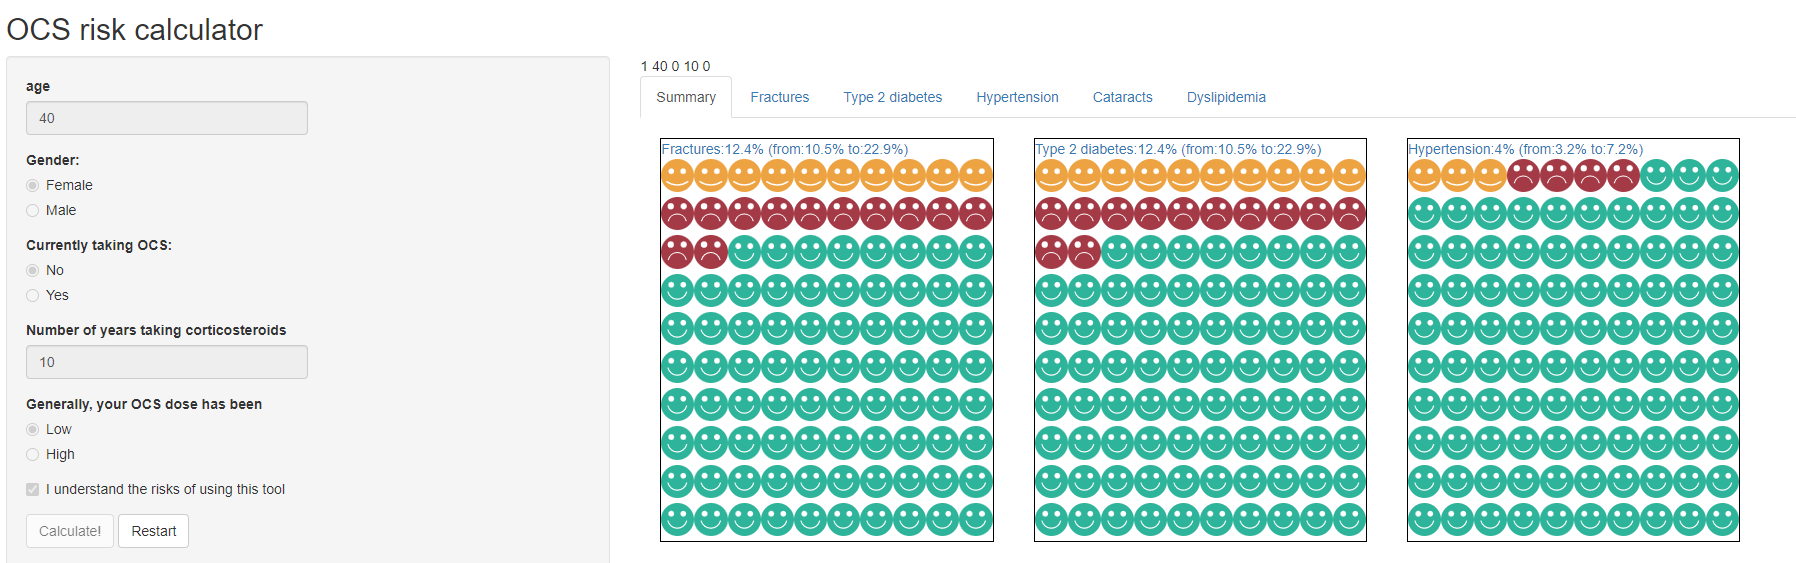
\includegraphics{AppExample.png}

\hypertarget{end-of-document}{%
\section{End of document}\label{end-of-document}}

\end{document}
